\documentclass{beamer}
\usetheme{Boadilla}
%typical packages
\usepackage{tikz,amsfonts,amsmath,pgfplots}
\setcounter{MaxMatrixCols}{20}
\usepackage{subfig}
\usepackage{bookmark}
% Include the algorithm packages
\usepackage{algorithm,algorithmic}
\usepackage{ifthen}
\usepackage{stmaryrd} % For \llbracket and \rrbracket


\usepackage{verbatim}
\usepackage{subcaption}
\usepackage{multirow}  % For the multirow functionality
\usepackage{lmodern}   % Optional, for improved font rendering


\usepackage{graphicx}

% Define the theorem environment
\newtheorem{theo}{Theorem}

\newenvironment{ftheo}[1][]
  {\begin{mdframed}\begin{theo}\ifthenelse{\equal{#1}{}}{}{\ (#1)}}
  {\end{theo}\end{mdframed}}

\usetikzlibrary{shapes,arrows,positioning}
\newcommand{\RR}{\mathbb{R}}
\newcommand{\norm}[2]{\left \lVert #1 \right \rVert_{#2}}
\newcommand{\abs}[1]{\left| #1 \right|}

\newtheorem{defn}{Definition}
% Define your custom colors
\definecolor{zzttqq}{rgb}{0.6,0.2,0}
\definecolor{ccqqqq}{rgb}{0.8,0,0}
\definecolor{zzqqqq}{rgb}{0.6,0,0}
\definecolor{qqqqff}{rgb}{0,0,1}

\usepackage{listings}
\usepackage{xcolor}
\definecolor{darkgreen}{RGB}{0,150,0} % A shade of dark green



\lstset{ 
  backgroundcolor=\color{white},   % set background color
  basicstyle=\ttfamily\small,      % basic font style
  keywordstyle=\color{blue},       % keyword style
  commentstyle=\color{darkgreen},      % comment style
  stringstyle=\color{red},         % string style
  numbers=left,                    % display line numbers
  numberstyle=\tiny\color{gray},   % line number style
  stepnumber=1,                    % the step between two line numbers
  numbersep=5pt,                   % how far the line-numbers are from the code
  frame=single,                    % adds a frame around the code
  tabsize=2,                       % sets default tabsize
  breaklines=true,                 % sets automatic line breaking
  breakatwhitespace=true           % breaks lines at whitespace
}
\captionsetup{justification=centering}
%\usepackage{showframe}


%\fvset{fontsize=\small, numbers=left} 

\newcommand{\mfile}[1]{
\begin{quote}
\VerbatimInput[frame=single,framesep=3mm,label=\fbox{\normalsize \textsl{\,#1\,}},fontfamily=courier,fontsize=\scriptsize]{#1}
\end{quote}
}

\newcommand{\Matlab}{\textsc{Matlab}\xspace}
\newcommand{\Octave}{\textsc{Octave}\xspace}
\newcommand{\Python}{\textsc{Python}\xspace}
\newcommand{\ipython}{\textsc{ipython}\xspace}
\newcommand{\numpy}{\textsc{numpy}\xspace}
\newcommand{\scipy}{\textsc{scipy}\xspace}
\newcommand{\matplotlib}{\textsc{matplotlib}\xspace}
\renewcommand{\thesubfigure}{\arabic{subfigure}}

\usepackage{pgf,tikz}
\usetikzlibrary{arrows}


\usepackage{listings}
\usepackage{xcolor}

\definecolor{codegreen}{rgb}{0,0.6,0}
\definecolor{codegray}{rgb}{0.5,0.5,0.5}
\definecolor{codepurple}{rgb}{0.58,0,0.82}
\definecolor{backcolour}{rgb}{0.95,0.95,0.92}

\lstdefinestyle{mystyle}{
    backgroundcolor=\color{backcolour},   
    commentstyle=\color{codepurple},
    keywordstyle=\color{magenta},
    numberstyle=\tiny\color{codegray},
    stringstyle=\color{codepurple},
    basicstyle=\ttfamily\footnotesize,
    breakatwhitespace=false,         
    breaklines=true,                 
    captionpos=b,                    
    keepspaces=true,                 
    numbers=left,                    
    numbersep=5pt,                  
    showspaces=false,                
    showstringspaces=false,
    showtabs=false,                  
    tabsize=2
}

\captionsetup{
  font=small,          % Select font size
  labelfont=bf,        % Select appearance of label
  margin=3em,          % Margin, left and right
  tableposition=top    % Formatting for captions above tables
}





\usepackage{mdframed}


\addtobeamertemplate{navigation symbols}{}{%
    \usebeamerfont{footline}%
    \usebeamercolor[fg]{footline}%
    \hspace{1em}%
    \insertframenumber/\inserttotalframenumber
}
\newcommand{\myfigure}[3]{
    \begin{figure}
        \centering
        \includegraphics[width=#1\textwidth]{#2}
        \caption{#3}
    \end{figure}
}
%typical tikz stuff
\tikzstyle{vertex}=[circle, draw, inner sep=0pt, minimum size=6pt,fill=white]
\newcommand{\vertex}{\node[vertex]}
\usepackage{pgf}
\usetikzlibrary{arrows}
\pagestyle{empty}
\definecolor{zzttqq}{rgb}{0.6,0.2,0}
\definecolor{uququq}{rgb}{0.25,0.25,0.25}
\definecolor{xdxdff}{rgb}{0.49,0.49,1}
\definecolor{qqqqff}{rgb}{0,0,1}


\title{AMR for Fluids and Other Applications}
\author{Stefano Fochesatto}
\institute{University of Alaska Fairbanks}
\date{\today}

\begin{document}
 \begin{frame}
\titlepage
\end{frame}


\beamertemplatenavigationsymbolsempty

\begin{frame}{Overview}
	\tableofcontents
\end{frame}


\section{Finite Element Method: Convergence Theorem}
\tableofcontents[currentsection]
  
  \begin{frame}
	\begin{definition}[Linear Variational Problem]
		Find $u \in H^1_{g_D}$ such that, 
		\begin{equation*}
		  a(u, v) = F(v) \text{ for all } v \in H^1_{0}.
		\end{equation*}
		Where $a(\cdot, \cdot): H^1(\Omega) \times H^1(\Omega) \rightarrow \mathbb{R}$ is a bilinear form, and $F(\cdot): H^1(\Omega) \to \mathbb{R}$ is a bounded linear form.
	\end{definition}

\end{frame}

\begin{frame}
	\begin{theo}[Cea's Lemma; Ex: Elman et al. 2005]
		Let $u$ be the solution to a linear variational problem on $H^1$ and $u_h$ be the finite element solution on $S^h$. If $a$ is continuous and coercive then there exists constants $\gamma, \alpha > 0$ such that,
		\begin{equation*}
		\norm{u - u_h}{H^1} \leq \frac{\gamma}{\alpha} \min_{v \in S^h}\norm{u - v}{H^1}.
	\end{equation*}
\end{theo}
\vfill
Let $\pi_h(u)$ be the interpolant of $u$ in $S^h$ then, 
\begin{equation*}
	\norm{u - u_h}{H^1} \leq \frac{\gamma}{\alpha} \norm{u -\pi_h(u)}{H^1}.
\end{equation*}
\end{frame}





  \begin{frame}
	  \begin{theo}[1; Ex: Elman et al. 2005]
		Let $T_h$ be a triangulation and $h_k$ be the largest length and $\theta_k$ be the minimum angle of $\triangle_k \in T_h$, then there exists some constant $C_2$
		\begin{equation*}
			\norm{\nabla(u - \pi_h(u))}{L_2}^2 \leq C_2\sum_{{\triangle_k}\in {T_h}} \frac{1}{\sin^2 \theta_k} h_k^2 \norm{D^2u}{\triangle_k}^2.
		   \end{equation*}
	  \end{theo}
	  \begin{itemize}
		\item By estimation of interpolation error and the Bramble-Hilbert Lemma. 
	  \end{itemize}
  \end{frame}

  \begin{frame}
	\begin{defn}[shape regularity; Ex: Elman et al. 2005]
		A sequence of triangulations $\{T_h\}$ is shape regular if there exists a minimum angle $\theta_* \neq 0$ such that every element in $T_h$ satisfies $\theta_T \geq \theta_*$.
	  \end{defn}
	  	\begin{figure}
	  \centering
	  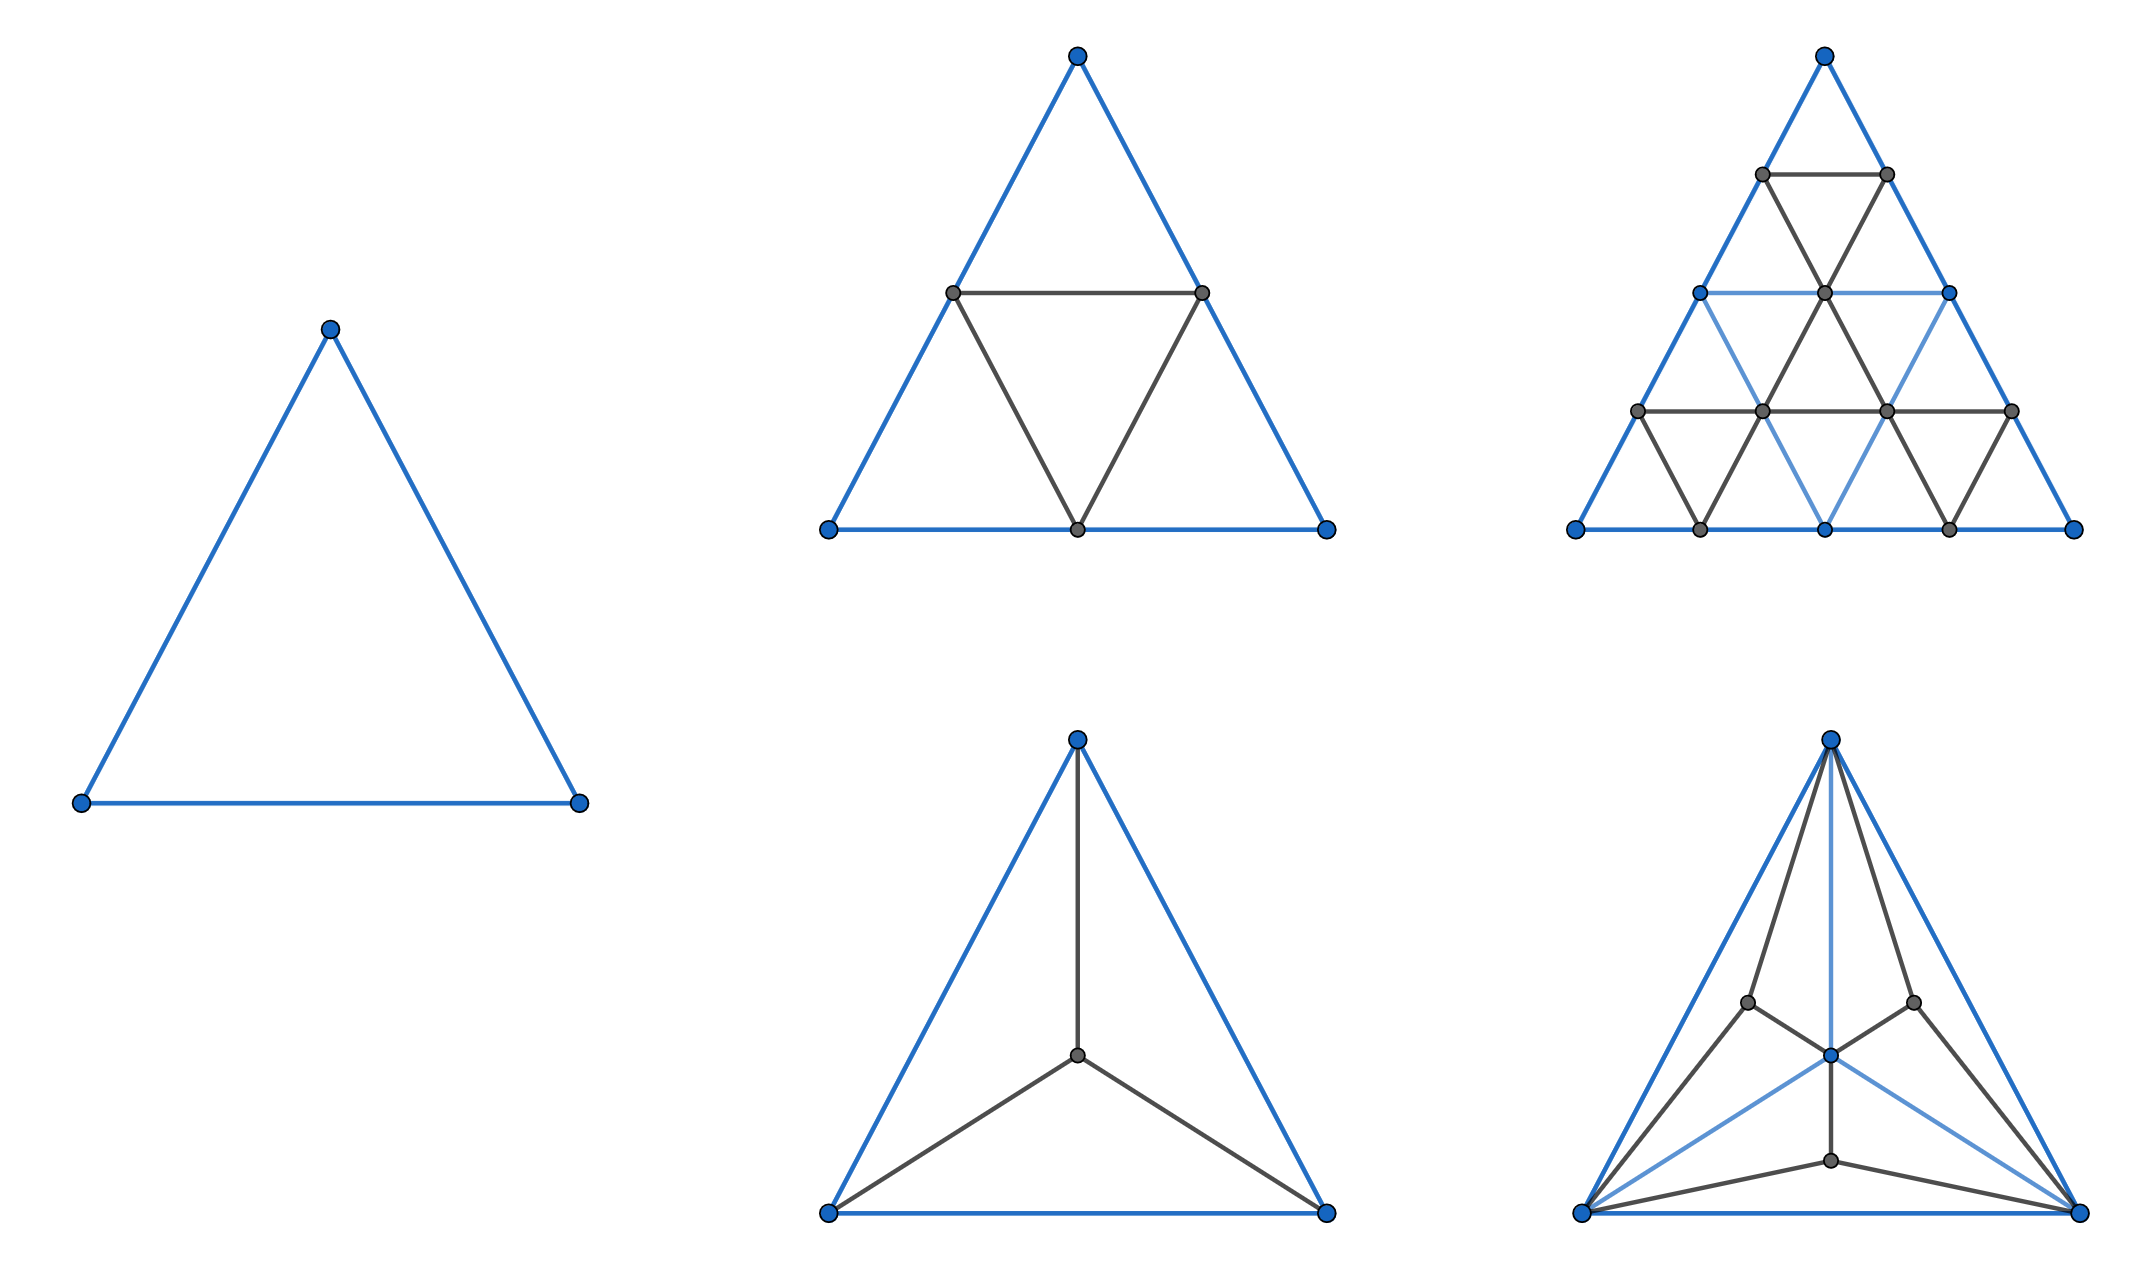
\includegraphics[width=.80\textwidth]{Figures/ShapeRegularity.png}
	  \caption*{Shape Regularity}
	\end{figure}
\end{frame}




  \begin{frame}
	\begin{itemize}
		\item All together \dots
	\end{itemize}
	\begin{align*}
		\norm{u - u_h}{H^1} &\leq \frac{\gamma}{\alpha}\norm{u - \pi_h(u)}{H^1} \qquad \text{(Céa's Lemma)},\\
		&\leq \frac{\gamma}{\alpha} \sqrt{1 + C_1} \norm{\nabla(u - \pi_h(u))}{L_2} \qquad \text{(Poincaré-Friedrichs)},\\
		&\leq \frac{\gamma}{\alpha} \sqrt{1 + C_1} \left(C_2\sum_{{\triangle_k}\in {T_h}} \frac{1}{\sin^2 \theta_k} h_k^2 \norm{D^2u}{\triangle_k}^2\right)^{\frac{1}{2}}
		\qquad \text{(Th.1)},\\
		&\leq  \frac{\gamma}{\alpha} \sqrt{(1 + C_1)C_2}  \frac{1}{\sin \theta_*} h\norm{D^2u}{\Omega} \qquad \text{(shape regularity)}.\\
		&= O(h).
	  \end{align*}
	  \begin{itemize}
		\item A different proof shows $O(h^2)$ for $L_2$.
	  \end{itemize}
  \end{frame}

  \begin{frame}
	\begin{itemize}
		\item A good $S^h$ minimizes the interpolation error. 
	\end{itemize}

		\begin{equation*}
			f(x, y) = \sqrt{1 - x^2} \quad \text{ on } \quad \Omega =  [-1, 1]^2
		\end{equation*}
		% Now I want to display two pngs side by side
		\begin{figure}
			\includegraphics[width=0.40\textwidth]{Figures/original.png}
			\includegraphics[width=0.40\textwidth]{Figures/adapted.png}
			\caption{Interpolation of anisotropic $f$ with roughly the same elements.}
		\end{figure}
  \end{frame}


  \begin{frame}
	\begin{itemize}
		\item A good refinement scheme should also focus on interpolation error. 
		% This figure needs a citation Frédéric Alauzet. Metric-based anisotropic mesh adaptation. https://pages.saclay.inria.fr/frederic.alauzet/cours/cea2010_V3.pdf, 2010.
	\end{itemize}

		\begin{center}
		\begin{figure}
				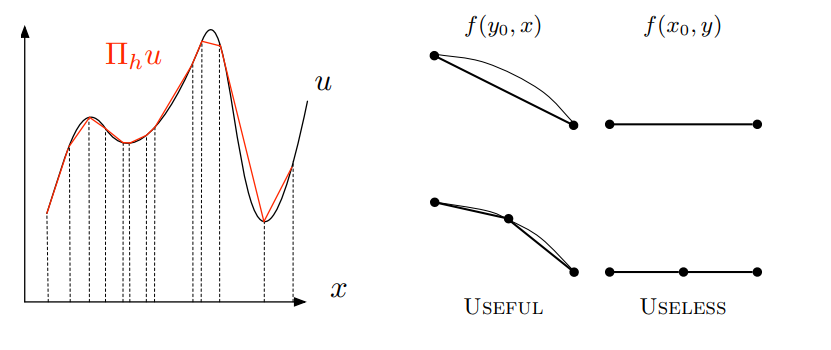
\includegraphics[width=\textwidth]{Figures/refinementinterp.png}
				\caption{(Alauzet, 2010)}
			\end{figure}
		\end{center}
  \end{frame}


\section{Adaptivity Schemes and Firedrake/PETSc Compatibility}
\tableofcontents[currentsection]


  \begin{frame}
	\frametitle{Tagging Schemes}
	\begin{enumerate}
		\item \textbf{Solve}: Compute the solution on the current mesh.
		\item \textbf{Estimate}: Estimate error for each element.
		\item \textbf{Tag}: Tag elements for refinement/coarsening based on estimate.
		\item \textbf{Refine}: Refine/coarsen mesh.
	\end{enumerate}
	
	\vfill
	
	\begin{itemize}
		\item Babuška-Rheinboldt error estimator (for Poisson), 
		\[
			\eta_K^2 =  h_K^2 \int_K  \, \Big| f + \nabla^2 u_h \Big|^2 \, dx + \frac{h_K}{2} \int_{\partial K \setminus \partial \Omega} \, \llbracket \nabla u_h \cdot \mathbf{n} \rrbracket^2 \, ds 
		\]

		\item Refine and coarsen in a way where error is equidistributed (Bangerth \& Rannacher, 2003)
	\end{itemize}
  \end{frame}

  \begin{frame}
	\begin{figure}
		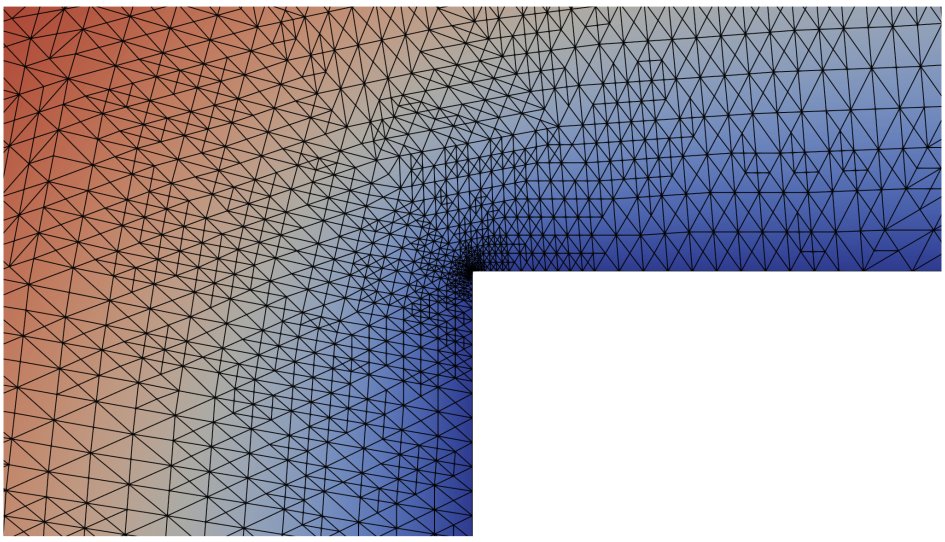
\includegraphics[width=\textwidth]{Figures/PoissonLshaped.png}
		\caption{L-Shaped Homogeneous Dirichlet Poisson Problem. (Farrell, 2024)}
	\end{figure}
	
  \end{frame}

  \begin{frame}[fragile]
	\begin{itemize}
		\item Mark and refine functionality is implemented in Firedrake via Netgen through ngsPETSc (Zerbinati et al. 2024). 2D and 3D
		\begin{lstlisting}[language=Python, basicstyle=\ttfamily\scriptsize]
			import netgen
			mesh = Mesh(ngmesh)
			...
			AdaptedMesh = mesh.refine_marked_elements(indicator)
		\end{lstlisting}
	\end{itemize}	
	\vfill
	\begin{itemize}
	\item The SBR algorithm (Plaza \& Carey. 1998) is available in PETSc with bindings in petsc4py (or VIAMR). 2D only
	\begin{lstlisting}[language=Python, basicstyle=\ttfamily\scriptsize]
		import VIAMR
		...
		AdaptedMesh = VIAMR.refinemarkedelements(mesh, indicator)
	\end{lstlisting}
	\vfill
	\item Neither implementation can coarsen, so not ideal for time dependent problems. 
	\end{itemize}
  \end{frame}


  \begin{frame}
  \frametitle{Metric Based Adaptation}
  \begin{itemize}
	\item Let $\Omega \subset  \RR^n$, and let $\textbf{M} = \{\mathcal{M}(x)\}_{x \in \Omega}$ be a Riemannian Metric Space, where $\mathcal{M}(x): \Omega \to \RR^{n \times n}$ is an SPD matrix.
	\vfill
	\item Notions of distance, volume, and angle are derived from $\textbf{M}$ and used during mesh generation to drive adaptivity.  
  \end{itemize}
  \begin{equation*}
	d_{\textbf{M}}(a,b) 
	= \int_{0}^{1} \| \boldsymbol{\gamma}'(t) \|_{\mathcal{M}} \, \mathrm{d}t 
	= \int_{0}^{1} \sqrt{ ab^T \, \mathcal{M}( a + t ab ) \, ab} \, \mathrm{d}t.
  \end{equation*}
  \begin{equation*}
	|K|_{\textbf{M}} = \int_{K} \sqrt{\det\mathcal{M}(x)} \, \mathrm{d}x\,.
  \end{equation*}
  \end{frame}


  \begin{frame}
	\frametitle{Geometric Interpretation}
	\begin{equation*}
		\mathcal{M}(x)^{-1/2} = U \Lambda^{-1/2} U^{-1}(x)\quad \text{ where } \quad \Lambda = I(\lambda_1^{-1/2}, \lambda_2^{-1/2}, ...)
	\end{equation*}
	\begin{figure}
		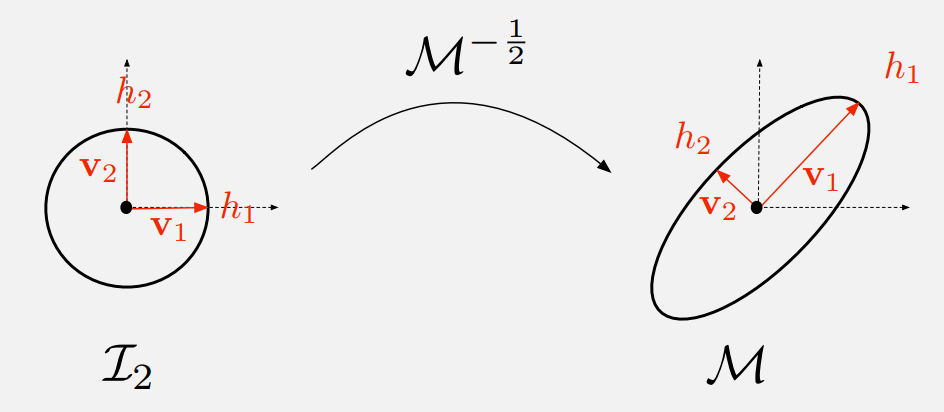
\includegraphics[width=\textwidth]{Figures/IdentityMap.png}
		\caption{(Alauzet, 2010)}
	\end{figure}
  \end{frame}

  \begin{frame}
	\frametitle{Geometric Interpretation}
	\begin{figure}
		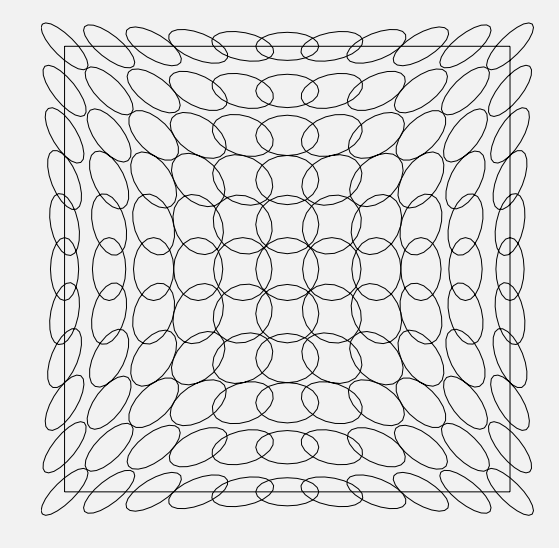
\includegraphics[width=.65\textwidth]{Figures/Ellipses.png}
		\caption{(Alauzet, 2010)}
	\end{figure}
  \end{frame}

  \begin{frame}
	\frametitle{Geometric Interpretation}
	\begin{figure}
		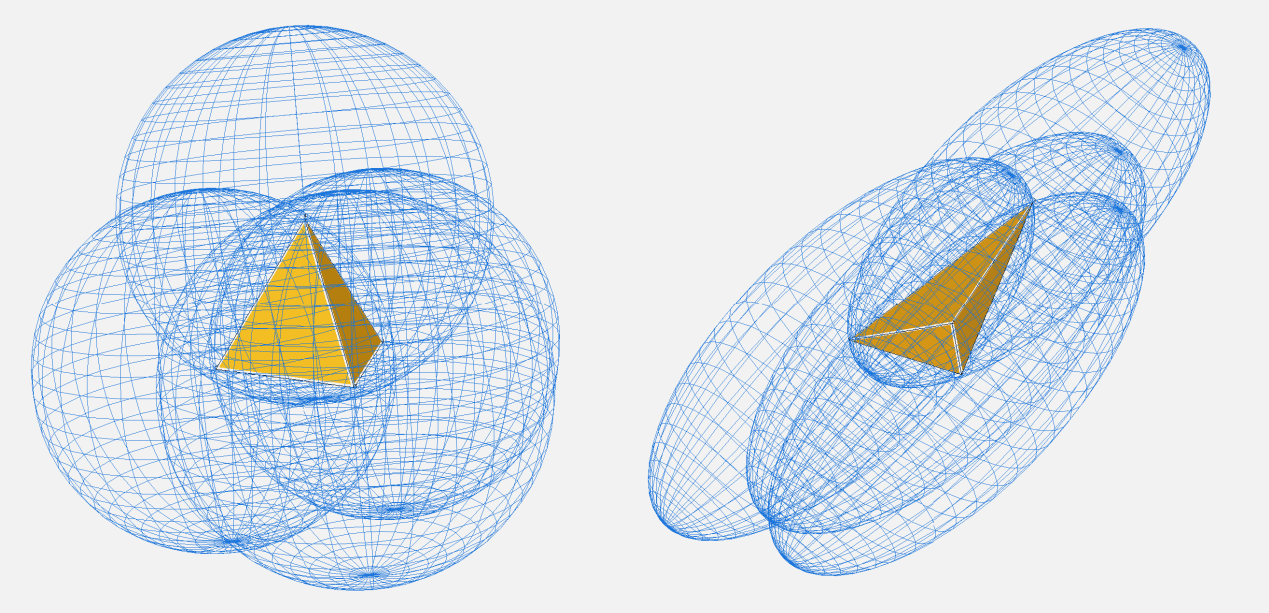
\includegraphics[width=.80\textwidth]{Figures/Tetra.png}
		\caption{(Alauzet, 2010)}
	\end{figure}
  \end{frame}


  \begin{frame}
	\frametitle{Isotropic Metrics and Operations}
	\begin{itemize}
		\item Isotropic metrics should treat each dimension the same,
		\begin{equation*}
			\mathcal{M}(x) = U(I\lambda(x))U^{-1}. 
		\end{equation*}
		\vfill
		\item We can intersect and average metrics to create new metrics. 
	\end{itemize}
	\begin{figure}
		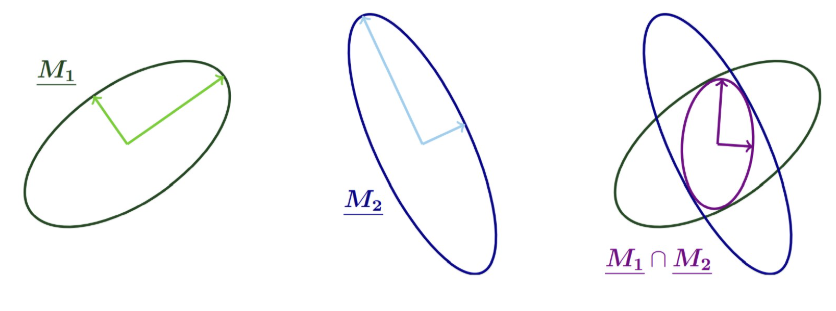
\includegraphics[width=.80\textwidth]{Figures/intersect.png}
		\caption{Metric Intersection (Wallwork, 2021)}
	\end{figure}
  \end{frame}



  \begin{frame}

	\begin{theo}[Alauzet, 2010]
		Let $u$ be a twice differentiable function on $\Omega$ with $H_u(x)$ its Hessian and let $\abs{H_u(x)} = U\abs{\Lambda}U^{-1}$. If $\mathcal{H}$ is a unit mesh of $\Omega$ generated with respect to the metric,
		\begin{equation*}
			\dfrac{c_n \abs{H_u}}{\epsilon}(x)
		\end{equation*}
		where $c_n$ depends on dimension of $\Omega$ then $\mathcal{H}$ is optimal within $\epsilon$ w.r.t controlling linear interpolation error in $L^\infty$ norm. 
	\end{theo}
	\vfill
	\begin{itemize}
		\item Methods exists for interpolating discretely defined metrics and recovering hessians from linear FE solutions. 
	\end{itemize}
  \end{frame}





  \begin{frame}[fragile]
	\begin{itemize}
		\item Parallel metric based adaptation is implemented in PETSc (Wallwork et al. 2022) and has been ported into Firedrake with the Animate library. 
		\vfill
		\begin{lstlisting}[language=Python, basicstyle=\ttfamily\scriptsize]
			import animate
			... 
			P1_ten = TensorFunctionSpace(mesh, "CG", 1)
			metric = RiemannianMetric(P1_ten)
			metric.set_parameters(metric_params)
			metric.compute_hessian(c)
			metric.normalise()
			adapted_mesh = adapt(mesh, metric)
		\end{lstlisting}
	\end{itemize}	
  \end{frame}

  \begin{frame}
	\frametitle{Time Dependent Metric Adaptation}
	\begin{enumerate}
		\item Perform hessian based adaptation on the initial time step.
		\item Solve the problem on a specified sub-interval.
		\item Compute the hessian based metric for each solution in the sub interval. 
		\item Intersect the metrics and adapt the mesh.
		\item Transfer the solution to the new mesh (interp or project)
		\item Re-solve the problem on the sub-interval.
		\item Repeat 2-6 on the next sub-interval until we reach the end of the simulation. 
	\end{enumerate}
  \end{frame}
  \begin{frame}
	\vfill
	Demo
	\vfill
  \end{frame}

  \begin{frame}
	\frametitle{Time Dependent Metric Adaptation (Metric Advection)}
	\begin{enumerate}
		\item Perform hessian based adaptation on the initial time step.
		\item Solve the fluid problem on a specified sub-interval.
		\item Solve the advection equation on the initial metric with fluid velocities for the duration of the sub-interval. 
		\item Intersect the metrics and refine the mesh.
		\item Re-solve the problem on the sub-interval.
		\item Repeat 2-5 on the next sub-interval until we reach the end of the simulation. 
	\end{enumerate}
  \end{frame}
  \begin{frame}
	\vfill
	Demo
	\vfill
  \end{frame}

  \begin{frame}
	\frametitle{SUPG Metric Advection}
	\begin{itemize}
		\item Solve for metric $M$ where, \[\frac{\partial m_{ij}}{\partial t} + u \cdot \nabla m_{ij} = 0.\]
		\item Implicit-Euler weak form, \[\int_\Omega \left( m^{n+1} \phi + \Delta t (u \cdot \nabla m^{n+1}) \phi \right) dx = \int_\Omega m^n \phi \, dx,\]
		\item SUPG stabilisation for CG finite elements modifies, \[\phi \rightarrow \phi + \tau \, u \cdot \nabla \phi.\]
		\item The amount of added diffusion is controlled by $\tau$.
		\item $\tau = \frac{h}{2|u|}$ for pure advection, $\tau = \frac{h|u|}{6K}$ for advection-diffusion.
		\end{itemize}
  \end{frame}



  





%%%%%%END%%%%%%%
\end{document}
